\documentclass[10pt, letter]{article}
\newcommand{\doctitle}{%
CS 7650 Natural Language Processing}
\newcommand{\bigO}{\ensuremath{\mathcal{O}}}
\usepackage{graphicx}
\usepackage{float}
\usepackage{listings}
\usepackage{comment}
\usepackage{fancyvrb}
\usepackage{booktabs}
\usepackage[usenames,dvipsnames]{color}
\usepackage[center]{caption}
\usepackage{algorithm}
\usepackage{algpseudocode}
\usepackage[margin=1in]{geometry}
\usepackage[usenames,dvipsnames]{color}
\usepackage{hyperref}
\hypersetup{
  colorlinks,
  citecolor=Violet,
  linkcolor=Black,
  urlcolor=Blue}
\begin{document}
\title{\textsc{Project \#1: Text Classification} \\ \textbf{\doctitle}}
  \author {Arvind Krishnaa Jagannathan \\ GT ID: 902891874}
   \date{January 24, 2013}
\maketitle

\section*{General Details and Project Structure}
The tarball submitted online has the following structure:
\begin{enumerate}
	\item A directory called \textit{src} which contains the code for the classifiers and for the plotting functionality.
	\item A directory called \textit{Response} which contains the response files of my ``main'' classifier and ``special'' classifier. My best ``main'' classifier was the \emph{Naive Bayes}, with a smoothing parameter of $\alpha = 10^{-3}$. I tried to improve on the Naive Bayes Classifier according to the paper \cite{rennie2003tackling} mentioned in the project specification. My best classifier from that was the \emph{Complement Naive Bayes} classifier, with the same smoothing parameter as above. (More details in following sections)
	\item A directory called \textit{generated\_files} which contain files where I have dumped the data produced by the classifiers. Some of the files in that directory are used to plot the data, and some are used to just to verify the metrics.
	\item Directories \textit{train}, \textit{dev} and \textit{test} contain the training, development and test data respectively.
	\item The files \textit{train.key}, \textit{dev.key} and \textit{scorer.py} are used to obtain the accuracy metrics of the training and development data.
	\item The file \textit{sentiment-vocab.tff} is the sentiment vocabulary \cite{wilson2009recognizing}
	\item The directory \textit{Report} contains the tex generated files for this Report. The file \textit{report.pdf} is available at the root of the tarball.
\end{enumerate}
Please consider this part of the report as a README for the project hierarchy.
\section{Data Processing}
I got 11,083 distinct tokens, some of them being nonsensical such as aat, ee and so on. These may be words misspelt or represent something specific to a domain. I have implemented it as a \textit{defaultdict} in Python (from collections.defaultdict).

\section{Word Lists}
\subsection*{Deliverable 1}
The Python file which does the rule based classification is \textit{RuleBasedClassifier.py}. The accuracy of the Rule-Based classifier I got was 22.55\%.
The response file for this deliverable is \textit{generated\_files/rule\_response}. Here is the resulting confusion matrix after running the \textit{scorer} script on the response file.
\begin{verbatim}
3 classes in key: set(['NEG', 'OBJ', 'POS'])
2 classes in response: set(['NEG', 'POS'])
confusion matrix
key     NEG     POS
NEG     19      18
OBJ     102     79
POS     14      43
----------------
accuracy: 0.2255 = 62/275
\end{verbatim}

\subsection*{Deliverable 2}
I performed the trial-and-error on the training data, and found that if I set the tuning parameter (absolute value of the difference between the number of positive and negative words) as $6$, I get the highest accuracy (I tried values from 1 to 10). I ran the ``Tweaked Classifier'' on the development data (Python file \textit{TweakedRuleBasedClassifier\_dev.py}) with this value of the tuning parameter and I got an accuracy rate of 65.45\%. The response file for this deliverable is \textit{generated\_files/tweaked\_response\_dev6} and here is the confusion matrix after running the \textit{scorer} script on the response file.
\begin{verbatim}
3 classes in key: set(['NEG', 'OBJ', 'POS'])
3 classes in response: set(['NEG', 'OBJ', 'POS'])
confusion matrix
key     NEG     OBJ     POS
NEG     1       33      3
OBJ     5       166     10
POS     0       44      13
----------------
accuracy: 0.6545 = 180/275
\end{verbatim}

\section{Naive Bayes}
\subsection*{Deliverable 3}
After training the Naive Bayes classifier, I applied it to the development data and got an accuracy of 72.00\%. The pertinent files are
\begin{itemize}
	\item \textbf{Python File for Naive Bayes}: \textit{NaiveBayesClassifier.py}
	\item \textbf{Response File}: \textit{generated\_files/naive\_response}
\end{itemize}
Here is the confusion matrix after running the \textit{scorer} script on the response file.
\begin{verbatim}
3 classes in key: set(['NEG', 'OBJ', 'POS'])
3 classes in response: set(['NEG', 'OBJ', 'POS'])
confusion matrix
key     NEG     OBJ     POS
NEG     12      24      1
OBJ     12      169     0
POS     8       32      17
----------------
accuracy: 0.7200 = 198/275
\end{verbatim}

\subsection{Smoothing}
\subsubsection*{Deliverable 4}
I tried values of $\alpha$ from $10^0$ to $10^{-7}$. The plot of the values of $\alpha$ versus the accuracy rate is given in Figure \ref{del4}. 
\begin{figure}[H]
  \centering
    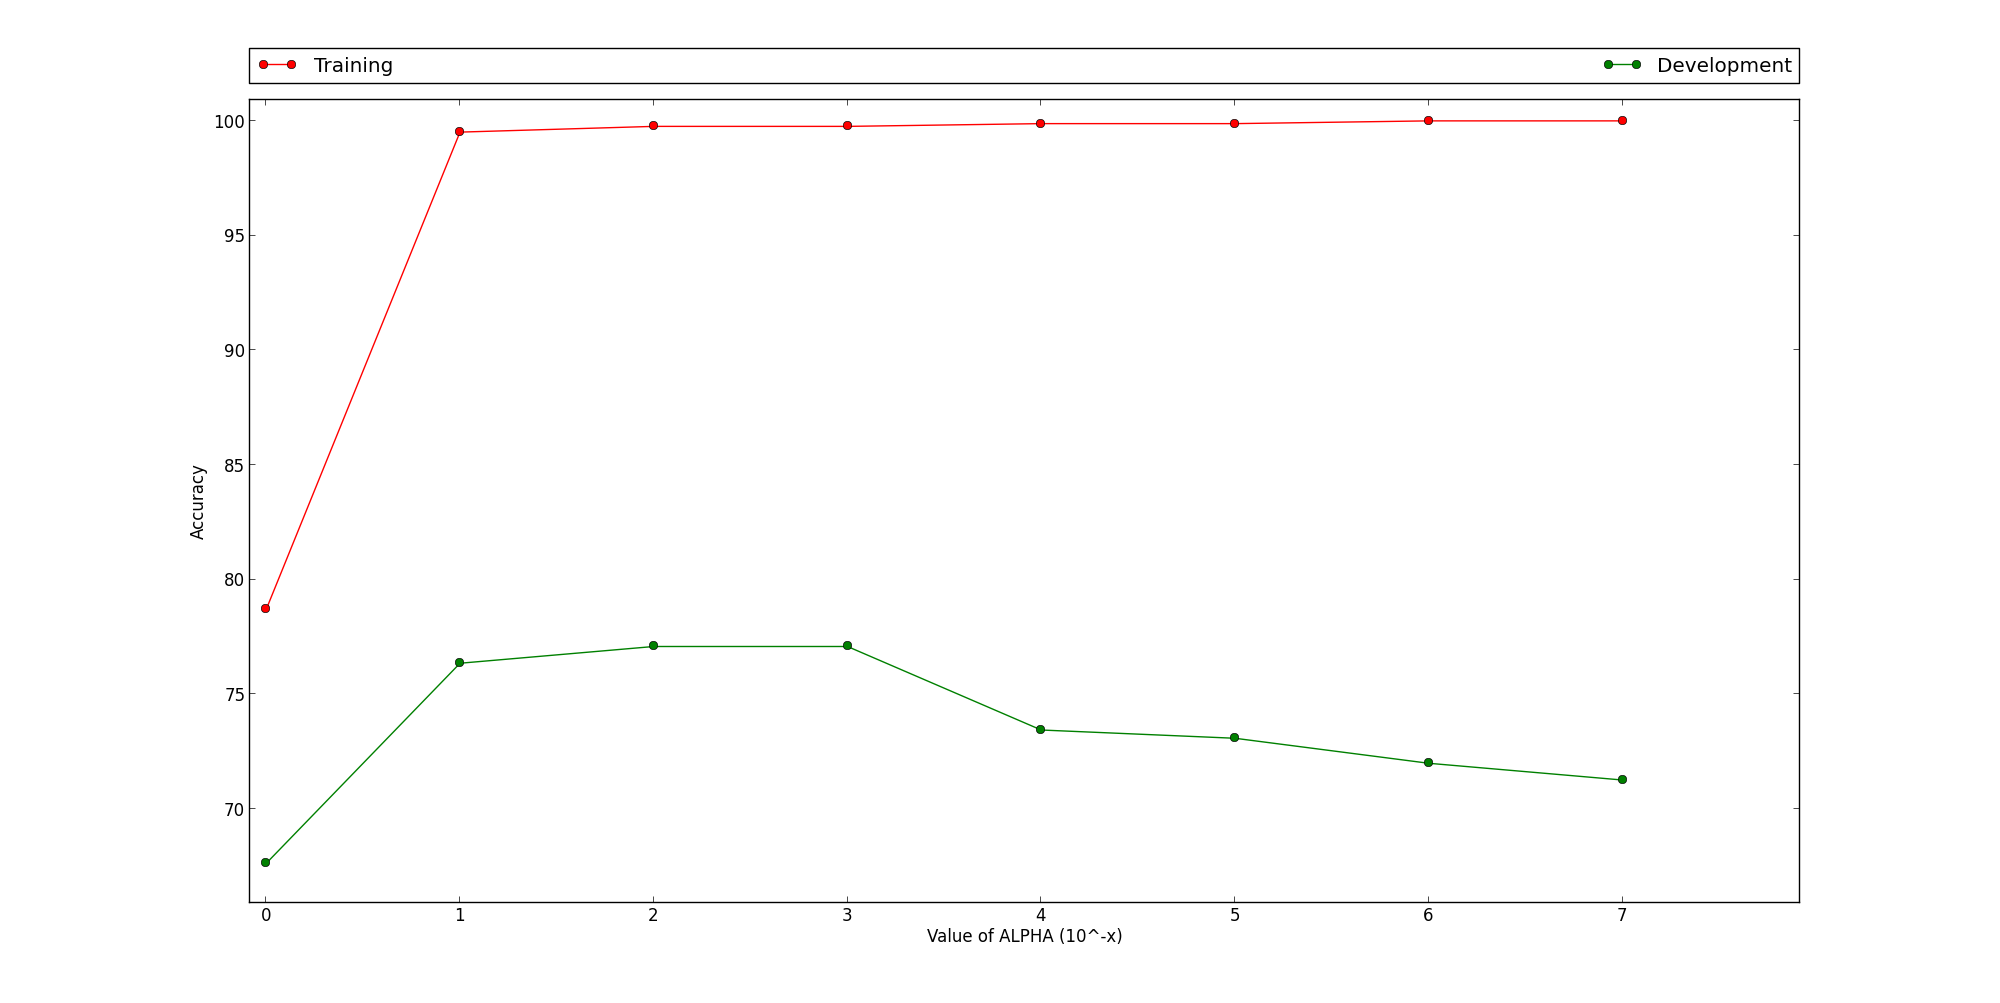
\includegraphics[scale=0.25]{images/deliverable_4}
    \caption{Plot of accuracy vs. $\alpha$ on both the training and development data}
  \label{del4}
\end{figure}

I got the best accuracy for the value of $\alpha = 10^{-3}$, which was 77.09\%.
The pertinent files are
\begin{itemize}
	\item \textbf{Python File}: \textit{SmoothingBayesClassifier.py}
	\item \textbf{Response File}: \textit{generated\_files/smoothing\_response\_6}
\end{itemize}
Here is the confusion matrix after running the \textit{scorer} script on the response file.
\begin{verbatim}
3 classes in key: set(['NEG', 'OBJ', 'POS'])
3 classes in response: set(['NEG', 'OBJ', 'POS'])
confusion matrix
key     NEG     OBJ     POS
NEG     19      16      2
OBJ     16      161     4
POS     6       19      32
----------------
accuracy: 0.7709 = 212/275
\end{verbatim}

\subsubsection*{Deliverable 5}
The plot of a random subset of the $\log(\theta)$ values for the the maximum and minimum values of $\alpha$ ($10^0$ and $10^{-7}$ respectively) is represented in Figure \ref{del5}.
\begin{figure}
  \centering
    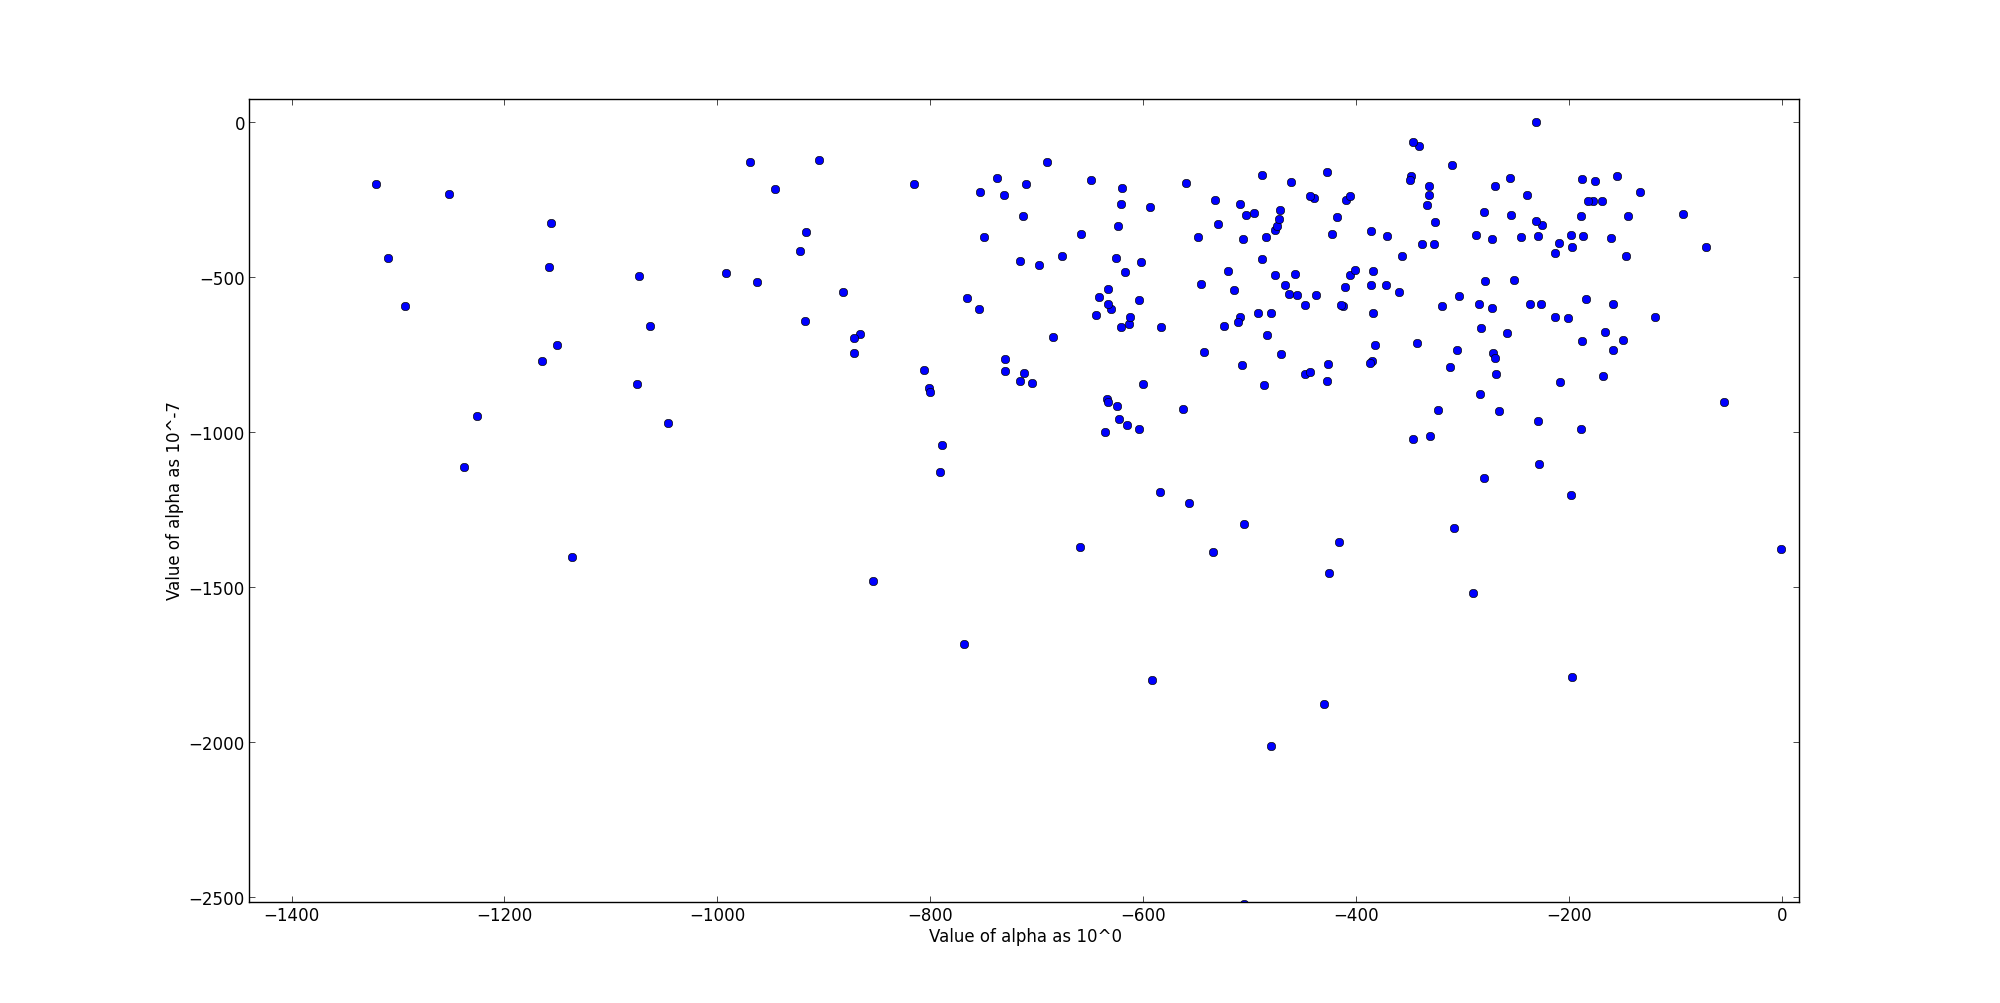
\includegraphics[scale=0.25]{images/deliverable_5}
    \caption{Plot of $\log{\theta}$ values for maximum and minimum values of the smoothing parameter.}
  \label{del5}
\end{figure}

The plotter script for this deliverable \textit{deliverable5.py} also computes the correlation coefficient, by using the spatial distance correlation method of Python's \textit{sciPy} \cite{scipy}. I got the value of the correlation as \textbf{0.8364}.
\subsubsection*{Explanation}
If the value of correlation had been 1, it would have meant that the $\log(\theta)$ values for the words were the same for both the maximum and minimum values of $\alpha$ are the same. A relatively high value like \textbf{0.8364} (quite close to the maximum value of 1) indicates that there is just a small variation in the weights assigned for each $\alpha$. In other words, the variance in the $\log(\theta)$ for different value of $\alpha$ is non-zero but quite small. However,  because of this small variance, the classification accuracy changes depending on the value of $\alpha$.

Moreover, the correlation indicates that if the value of $\alpha$ is very small $10^{-7}$ (which is almost 0 practically), the smoothing effect is almost null and the classifer is effectively the same as the Naive Bayes. With a very large value of $\alpha$ ($10^0$ = $1$, large is a relative term of course), we introduce a bias in the classifer. This is to our advantage with respect to the dataset of this particular project, because the distribution of classes in the training as well as the development data is the same (there is significantly more documents marked \textsc{Obj} in training as well as testing). And clearly the best accuracy will result in a value of $\alpha$ somewhere halfway between the maximum and minimum value, which is true in my case as well.

\subsection*{Deliverable 6}
The words which are most predictive of positive versus negative text from the training data are:
\begin{enumerate}
	\item city
	\item religious	
	\item republican	
	\item police
	\item enjoy
\end{enumerate}
Only the word \textit{enjoy} appears in the sentiment vocabulary\\
The words which are most predictive of negative versus positive text from the training data are:
\begin{enumerate}
	\item poker
	\item games	
	\item rated	
	\item century
	\item documentary
\end{enumerate}
None of these words appear in the sentiment vocabulary. These words have been determined as well as checked for presence in the sentiment vocabulary by the Python scripts \textit{MostPredictiveWords\_Positive\_Negative\_Bayes.py} and \textit{MostPredictiveWords\_Negative\_Positive\_Bayes.py} and have been written into the files \textit{generated\_files/top5pos\_neg} and \textit{generated\_files/top5neg\_pos} respectively.

\section{Perceptron}
I implemented the perceptron by representing each document's feature function as a sparse array in \textit{numpy}, whose size = number of distinct tokens in the training data. I was able to obtain a significant performance boost this way compared to representing it as a normal array (I was able to do 30 passes on training data in 40 seconds using \textit{numpy} as opposed to 2 passes per minute using the default array structure). I am pretty confident of my implementation, but I get a low accuracy rate on development data, (best case 60\% worst case 48\%).

\subsection*{Deliverable 7}
After making 30 passes on the training and development data, the plot for the accuracy vs. number of iterations is represented in Figure \ref{del7}
\begin{figure}
  \centering
    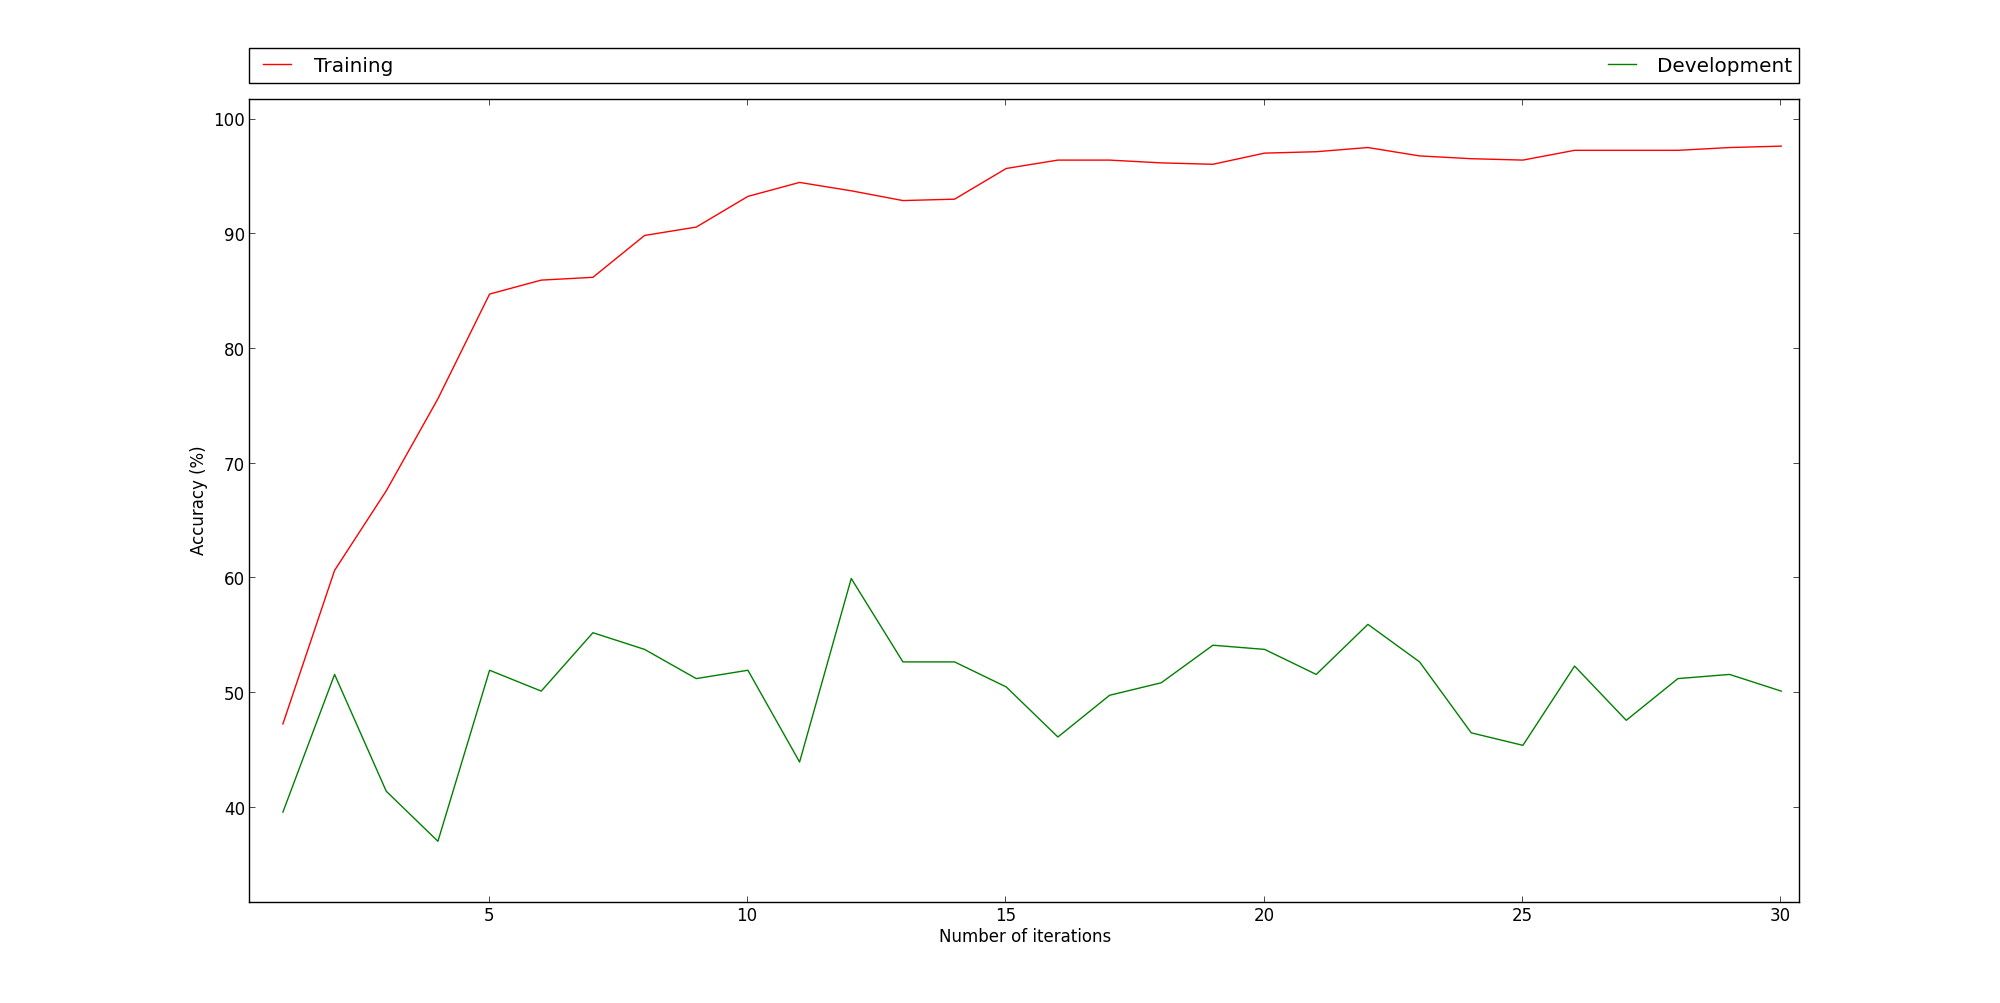
\includegraphics[scale=0.25]{images/deliverable_7}
    \caption{Plot of accuracy vs. number of iterations on training and development data}
  \label{del7}
\end{figure}
The final confusion matrix for the training and development data are as follows:
\begin{verbatim}
Training Perceptron Response
-------------------------------------
3 classes in key: set(['NEG', 'OBJ', 'POS'])
3 classes in response: set(['NEG', 'OBJ', 'POS'])
confusion matrix
key     NEG     OBJ     POS
NEG     137     4       2
OBJ     5       509     2
POS     2       4       157
----------------
accuracy: 0.9769 = 803/822

Development Perceptron Response
---------------------------------------------
3 classes in key: set(['NEG', 'OBJ', 'POS'])
3 classes in response: set(['NEG', 'OBJ', 'POS'])
confusion matrix
key     NEG     OBJ     POS
NEG     3       24      10
OBJ     14      112     55
POS     3       31      23
----------------
accuracy: 0.5018 = 138/275
\end{verbatim}
Pertinent files for this part of the project are:
\begin{itemize}
	\item \textbf{Python file for the Perceptron}: \textit{PerceptronClassifier\_proper.py}
	\item \textbf{Python file for plotting}: \textit{deliverable7.py}
	\item \textbf{File which has the accuracy measure after each pass}: 
		\begin{enumerate}
			\item For training data: \textit{generated\_files/training\_perceptron\_data\_akj}
			\item For development data: \textit{generated\_files/development\_perceptron\_data\_akj}
		\end{enumerate}
	\item \textbf{Response File for the last pass}: 
	\begin{enumerate}
			\item For training data: \textit{generated\_files/training\_perceptron\_response\_akj}
			\item For development data: \textit{generated\_files/perceptron\_response\_akj}
		\end{enumerate}
\end{itemize}

\subsection*{Deliverable 8}
The words which are most predictive of positive versus negative text from the training data are:
\begin{enumerate}
	\item about
	\item enjoy	
	\item china	
	\item recommend
	\item fitzgerald
\end{enumerate}
Only the words \textit{enjoy} and \textit{recommend} appear in the sentiment vocabulary\\
The words which are most predictive of negative versus positive text from the training data are:
\begin{enumerate}
	\item abandonment
	\item destruction
	\item death
	\item the
	\item at
\end{enumerate}
The words \textit{abandonment}, \textit{destruction} and \textit{death} occur in the sentiment vocabulary. 

These words have been determined as well as checked for presence in the sentiment vocabulary by the Python script \textit{MostPredictiveWords\_Positive\_Negative\_Negative\_Positive\_Perceptron.py} (a single file with a ridiculous name I formed due to lack of imagination) and have been written into the files \\ \textit{generated\_files/top5pos\_neg\_perceptron} and \textit{generated\_files/top5neg\_pos\_perceptron} respectively.

Two interesting observations I derive from the results of deliverables 8 and 6. 
\begin{enumerate}
	\item The perceptron being a error-driven approach, is able to identify the words which contribute to the class of a particular document, whereas the Naive Bayes method purely looks at the statistical occurrences of the words. Thus, I believe that had the documents in the development data have almost the same number of \textsc{Obj}, \textsc{Pos} and \textsc{Neg} documents, the perceptron classifier would have outperformed the Naive Bayes.
	\item The top 5 list of the perceptron classifer has more words in the sentiment vocabulary than the Naive Bayes. This also substantiates the above point. As an aside, the word \textit{enjoy} is the only common one between the two classifiers' top 5 lists.
\end{enumerate}

\section{Averaged Perceptron}
\subsection*{Deliverable 9}
I have performed the weight averaging after every iteration over the training data. After making 30 passes on the training and development data, the plot for the accuracy vs. number of iterations is represented in Figure \ref{del9}
\begin{figure}
  \centering
    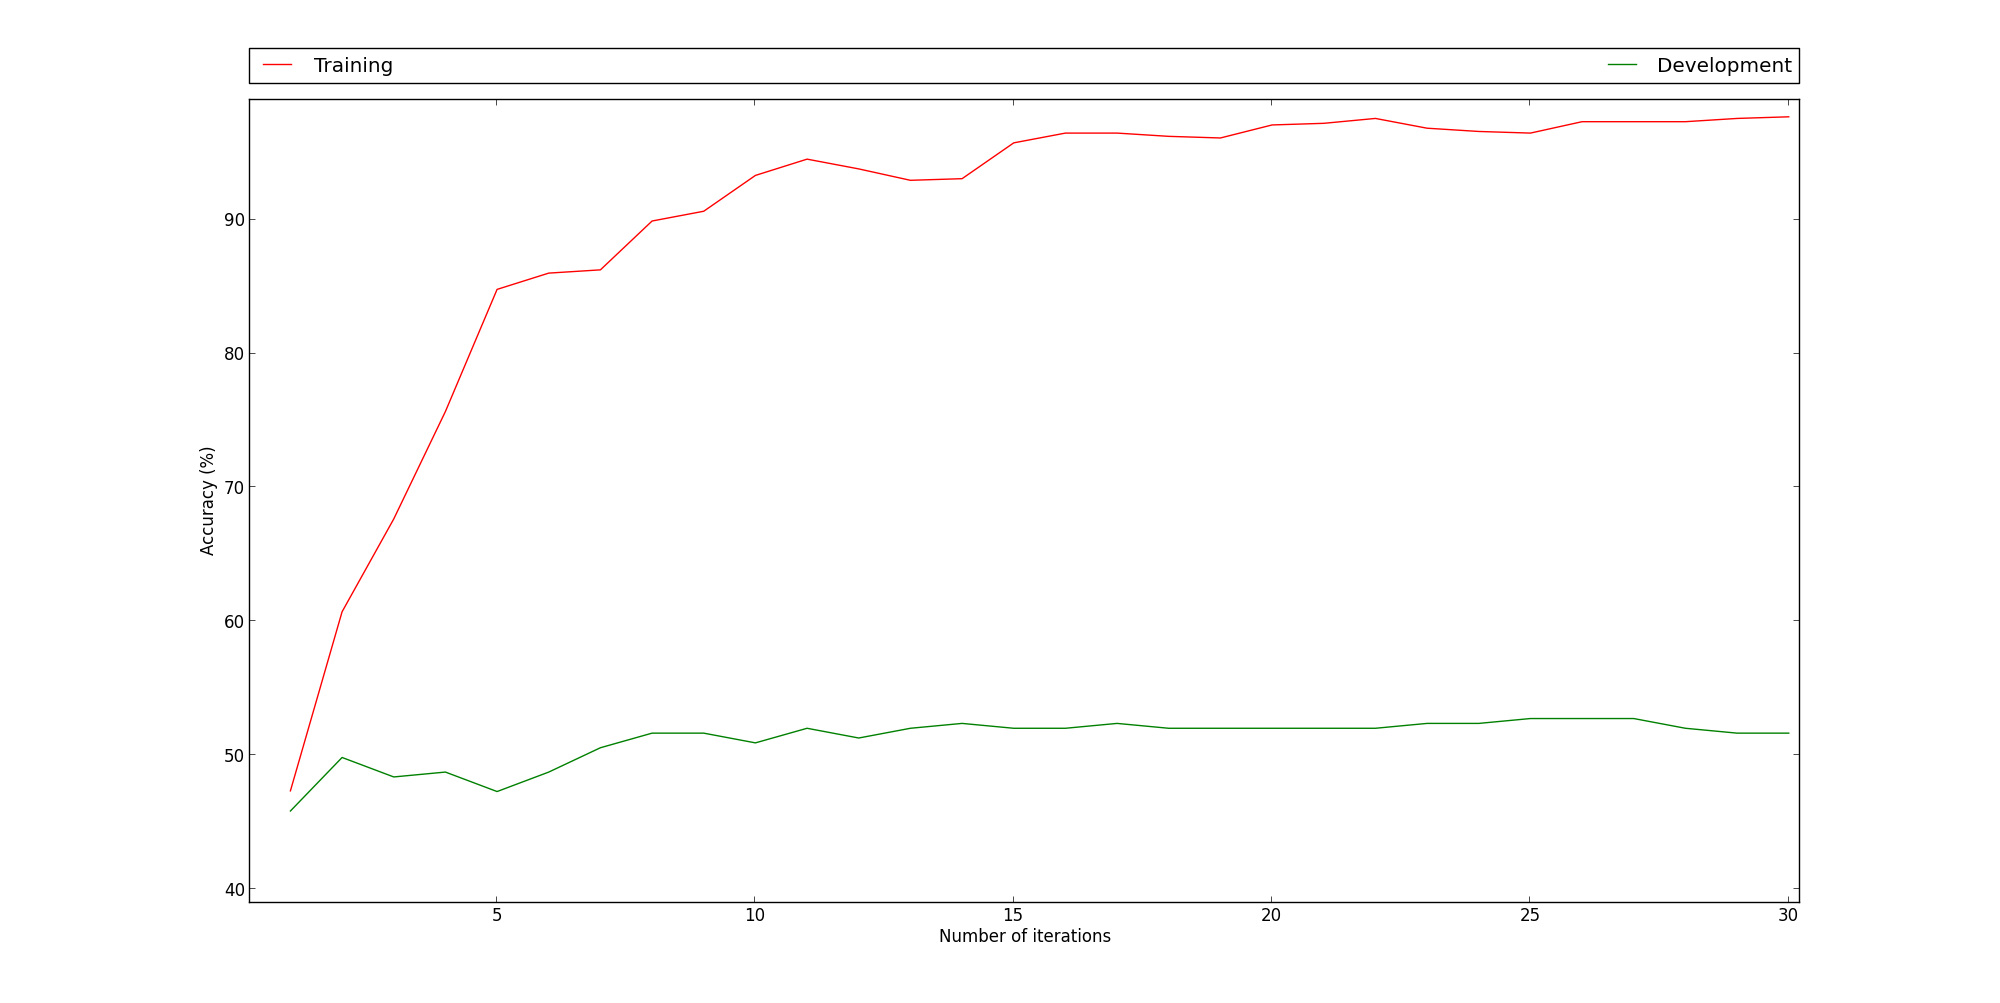
\includegraphics[scale=0.25]{images/deliverable_9}
    \caption{Plot of accuracy vs. number of iterations on training and development data - Averaged Perceptron}
  \label{del9}
\end{figure}
It is very noticeable that the accuracy measure (on the development data) does not fluctuate as much (a.k.a thrash) as it did without weight averaging and is visibly ``smoother''.

The final confusion matrix for the training and development data are as follows:
\begin{verbatim}
Averaged Training Perceptron Response
-------------------------------------
3 classes in key: set(['NEG', 'OBJ', 'POS'])
3 classes in response: set(['NEG', 'OBJ', 'POS'])
confusion matrix
key     NEG     OBJ     POS
NEG     137     4       2
OBJ     5       509     2
POS     2       4       157
----------------
accuracy: 0.9769 = 803/822

Averaged Development Perceptron Response
-------------------------------------
3 classes in key: set(['NEG', 'OBJ', 'POS'])
3 classes in response: set(['NEG', 'OBJ', 'POS'])
confusion matrix
key     NEG     OBJ     POS
NEG     4       24      9
OBJ     15      119     47
POS     3       35      19
----------------
accuracy: 0.5164 = 142/275

\end{verbatim}
Pertinent files for this part of the project are:
\begin{itemize}
	\item \textbf{Python file for the Perceptron}: \textit{AveragedPerceptronClassifier\_proper.py}
	\item \textbf{Python file for plotting}: \textit{deliverable9.py}
	\item \textbf{File which has the accuracy measure after each pass}: 
		\begin{enumerate}
			\item For training data: \textit{generated\_files/training\_perceptron\_data\_akj}
			\item For development data: \textit{generated\_files/averaged\_development\_perceptron\_data\_akj}
		\end{enumerate}
	\item \textbf{Response File for the last pass}: 
	\begin{enumerate}
			\item For training data: \textit{generated\_files/training\_perceptron\_response\_akj}
			\item For development data: \textit{generated\_files/averaged\_perceptron\_response\_akj}
		\end{enumerate}
\end{itemize}

\subsection*{Deliverable 10}
The plot of Perceptron weights vs. $\log(\theta)$ from Naive Bayes (for $\alpha = 10^{-3}$) is a very interesting one. The graph in Figure \ref{del10} is a random sampling of all the points. Notice that there are several data points for which either x or the y value is 0. Such points (by definition) are not considered for computing correlation \cite{scipy}.

\begin{figure}
  \centering
    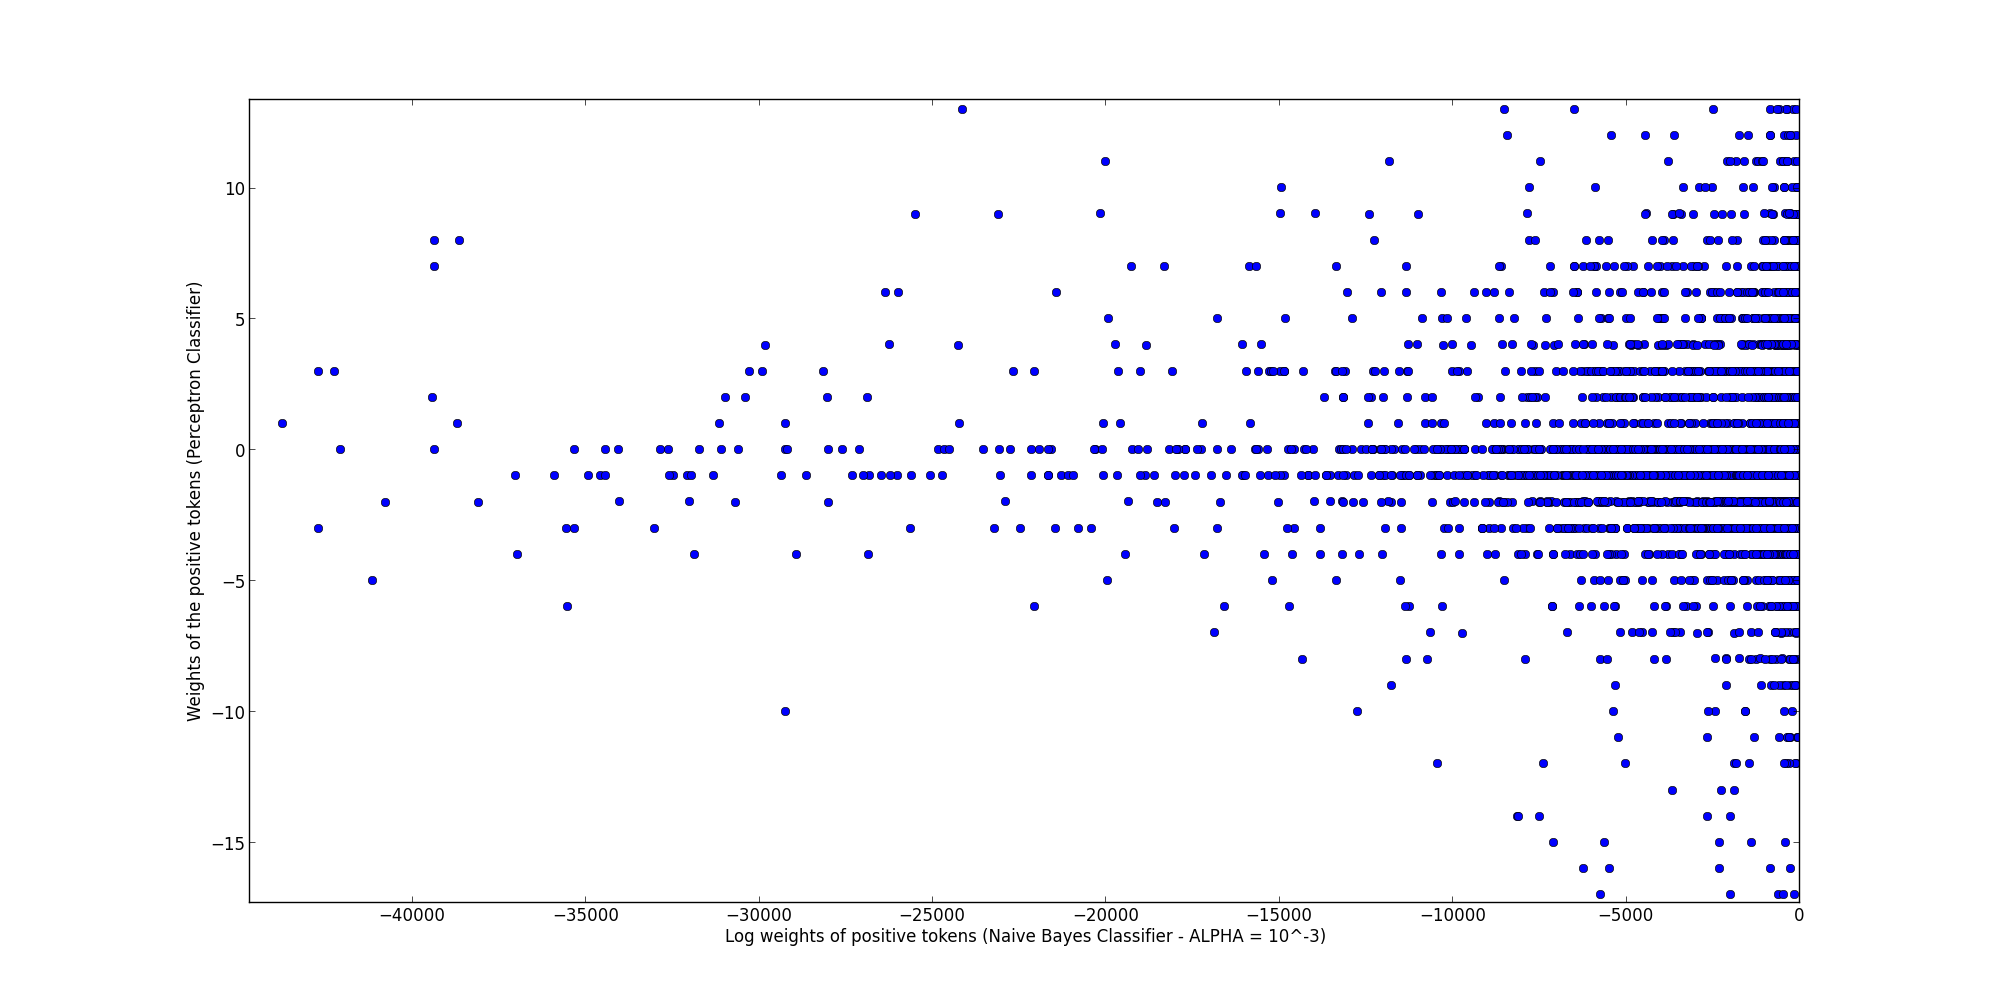
\includegraphics[scale=0.25]{images/deliverable_10}
    \caption{Averaged Perceptron weights vs. $\log(\theta)$ from Naive Bayes (for $\alpha = 10^{-3}$)}
  \label{del10}
\end{figure}

The correlation measure, found similar to deliverable 5 came out to be \textbf{0.983837736138}. This shows that for all the ``interesting points'' (notice the clustering just before the line $x=0$, around the imaginary line $x=y$), the weights assigned by both the Averaged Perceptron as well as the Smoothing Naive Bayes classifers are almost identical. Due to the poorly assigned scales for the axes by \textit{matplotlib} (and my inability to correct it), the above mentioned clustering may not be obvious. Figure \ref{del11} provides a highly zoomed in version of the above plotting. Note that the line in red represents the line $x=y$ and since its zoomed in (I think about 1000\% zoom) the distance of points from the line is actually miniscule (as indicated in the diagram almost 0).

\begin{figure}
  \centering
    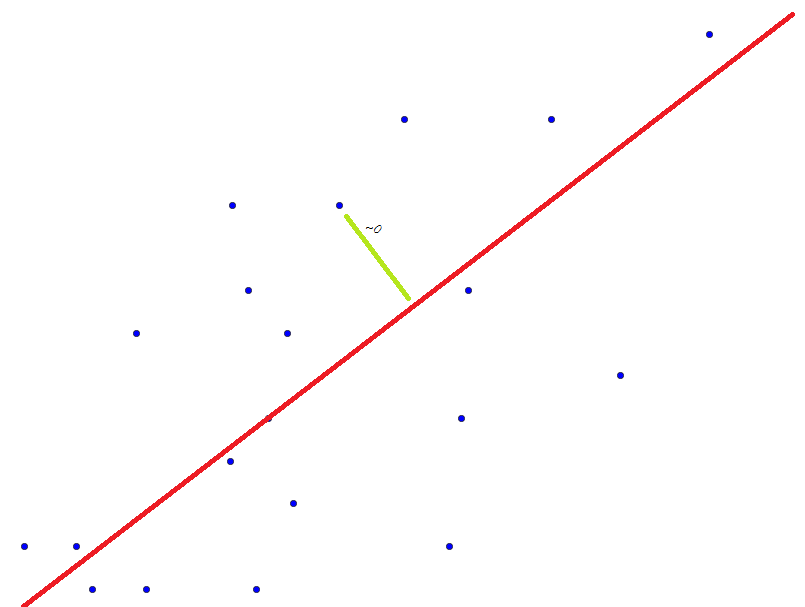
\includegraphics[scale=0.25]{images/deliverable_10_1}
    \caption{Figure \ref{del10} zoomed in}
  \label{del11}
\end{figure}


I thought such a high correlation would translate in more words in their respective top 5 lists to be common, but I guess very small floating point differences must exist. So I think that both the Naive Bayes as well as the Perceptron classifiers are able to almost identically separate the tokens into the three classes, the differences arise primarily because of the nature of the data set.

\section{Making it Better}
\subsection*{Deliverable 11}
I implemented all the methods to improve the Naive Bayes classifier, from the paper provided as reference \cite{rennie2003tackling} mainly because they were really easy to understand and fairly straight forward to implement. I believed that the accuracy rates of each of these techniques would be significantly higher than that of the Naive Bayes (NB). I expected that the Transformed Weight-Normalized Complementary Naive Bayes (TWCNB) method would give the highest accuracy. My rationale was as follows:
\begin{enumerate}
	\item It takes into account the probability of a token appearing in classes other than the class under consideration. (CNB)
	\item It performs weight normalization of the $\log(\theta)$ weights (although I have done the same in my implementation of the Naive Bayes classifier itself) (WCNB)
	\item It takes into account length of each document as well as the ``importance'' measure of a token (an IDF measure), meaning frequently occurrring words will not be given higher weight. (informally, TWCNB = NB + CNB + WCNB + IDF measure)
\end{enumerate}
However, when I ran the classifiers on the development data, my accuracy rates were in the following order,

	\textbf{Best Smoothened NB $\sim$ Complement NB \textgreater WCNB $\sim$ TWCNB \textgreater NB}

I assume that the improvement techniques did not do much to improve the accuracy of the Smoothened Naive Bayes, simply because both the training data and development data are similarly biased towards the \textsc{Obj} class. Even in the paper it was mentioned that Naive Bayes would drastically degrade if the development data had a different bias (or no bias) when compared to the training data. To test this, I trained the classifiers on the training data and then applied them on the development data. However, I decided to interchange every document marked as \textsc{Obj} into \textsc{Pos} and vice-versa in the \textit{dev.key} file. Then I ran the scorer script on the response files of each classifier. I expected all of them to perform poorly (of course), but I thought the classifiers using weight normalization would perform better (even in such perplexing scenarios). And I was proven right, the new accuracy measures were ordered as,

	\textbf{Complement NB $\sim$ TWCNB \textgreater WCNB $\sim$ Best Smoothened NB \textgreater NB}

This shows that in general, TWCNB would outperform Naive Bayes. Pertinent files can be found inside \textit{generated\_files/test} directory

\section{Bake Off}
\subsection*{Deliverable 12}
The best system from the main part of the project was the smoothened Naive Bayes (!). I ran it on the test data (Best\_Smoothing\_Bayes\_test\_data.py) and the response is the file \textbf{jagannathan-arvind\_krishnaa.main.response} inside the \textit{Response} directory.

\subsection*{Deliverable 13}
The best system from the making it better part of the project was the complement Naive Bayes. I ran it on the test data (Best\_Better\_Bayes1\_test\_data.py) and the response is the file \textbf{jagannathan-arvind\_krishnaa.special.response} inside the \textit{Response} directory.

\bibliographystyle{unsrt}
\bibliography{myrefs}
\end{document}